\documentclass[11pt]{article}
\usepackage[a4paper,margin=2.5cm]{geometry}
\usepackage{amsmath,amssymb,amsthm,array,booktabs,graphicx,microtype,float}
\usepackage[numbers]{natbib}
\usepackage{hyperref}
\usepackage{xr}
\hypersetup{hidelinks}
\externaldocument[M-]{main}
\renewcommand{\bibfont}{\footnotesize}
\floatstyle{ruled}
\newfloat{algorithm}{tbp}{loa}
\floatname{algorithm}{Algorithm}

\newtheorem{theorem}{Theorem}
\newtheorem{proposition}{Proposition}
\newtheorem{corollary}{Corollary}
\newtheorem{lemma}{Lemma}
\newtheorem{remark}{Remark}

\title{Supplementary Material for\\
Hierarchical Convexity-Run Decomposition:\\
Finite-Sample Chord-Lobe Recovery and Interpretable LC--MS Transfer}
\author{Saveliy Baturin\\Independent Researcher}
\date{Draft \today}

\begin{document}
\maketitle

This supplement contains optional scan and post-selection theory, complete
secondary experimental results, and detailed proof edges.  Numbered references
to theorems, figures, and tables in the main article use the main-article
numbering.

\section{Template scans for chord lobes}

These are conservative sup-norm certificates.  They are not sharp detection
boundaries when location and scale are unknown.  Modern multiscale shape tests
and scan statistics provide the relevant calibration and minimax comparison
targets \citep{dumbgen2001multiscale,ariascastro2005geometric,
sharpnack2018scan}.

The complete HCRD shapes also admit a sharper finite-dictionary statement.
Let $P$ project onto $\operatorname{span}\{\mathbf 1,x\}$ and let $M\ge2$ and
$v_1,\ldots,v_M\in\operatorname{range}(I-P)$ be unit-norm, oriented lobe
templates.  They may be fixed in advance or extracted from an independent
guide replicate; in the latter case all statements below are conditional on
that guide.  Write $\rho_m=\max_{k\ne m}\langle v_k,v_m\rangle<1$.

\begin{theorem}[Lobe-dictionary detection, localisation, and lower bound]
\label{thm:lobe-scan}
For $Y=g+\epsilon$, $g\in\operatorname{range}(P)$ and
$\epsilon\sim N(0,\sigma^2I)$, the scan
\begin{equation}
 S=\max_{1\le m\le M}\frac{\langle v_m,Y\rangle}{\sigma}
\end{equation}
has level at most $\alpha$ at threshold
$t_\alpha=\sqrt{2\log(M/\alpha)}$.  Under
$Y=g+\sigma\mu v_m+\epsilon$, its miss probability is at most $\beta$ whenever
\begin{equation}
 \mu\ge t_\alpha+\sqrt{2\log(1/\beta)}.
\end{equation}
Moreover, the maximiser of the scan equals $m$ with probability at least
$1-\delta$ if
\begin{equation}
 \mu(1-\rho_m)>2\sqrt{2\log(2M/\delta)}.
\end{equation}
Conversely, if the $v_m$ are orthonormal and $\alpha+\beta<1$, no level-$\alpha$
test has power greater than $1-\beta$ uniformly over all $M$ alternatives when
\begin{equation}
 e^{\mu^2}-1\le4M(1-\alpha-\beta)^2.
\end{equation}
Under a uniform unknown index, every index estimator also has mean error at
least $1-(\mu^2+\log2)/\log M$.  Thus both detection and localisation have
critical standardised lobe norm of order $\sqrt{\log M}$.  Over the stated
orthonormal subclass, the scan therefore matches the lower-bound order
$\sqrt{\log M}$, with an explicit constant gap; this is not a minimax claim
for every correlated HCRD dictionary.
\end{theorem}
\begin{proof}
Under the null each scan coordinate is standard Gaussian, possibly correlated,
so a Gaussian tail bound and union bound give
$\Pr(S>t_\alpha)\le M e^{-t_\alpha^2/2}=\alpha$.  Under the stated alternative,
the true coordinate is $N(\mu,1)$, which proves the miss bound.  With probability
at least $1-\delta$, all $M$ centred coordinates have magnitude at most
$u=\sqrt{2\log(2M/\delta)}$.  The true coordinate then exceeds every competitor
when $\mu-u>\mu\rho_m+u$.

For the lower bound, restrict the affine nuisance to $g=0$ and mix the $M$
orthogonal alternatives uniformly.  Its chi-squared divergence from the null is
$(e^{\mu^2}-1)/M$, hence total variation is at most one half of its square root.
The displayed condition makes average power at most $1-\beta$, so at least one
alternative has no greater power.  Finally the pairwise Gaussian
Kullback--Leibler divergence is $\mu^2$; Fano's inequality
\citep{cover2006elements} gives the localisation claim.
\end{proof}

The theorem concerns fixed or independently selected residual shapes.  It does
not make the discontinuous same-replicate knot selector innocuous, and its
orthogonal lower-bound subclass is a benchmark rather than a claim that all
HCRD lobes are mutually orthogonal.

The finite dictionary is not the mathematical end point: location, scale, and
asymmetry are naturally continuous.  Let $\Theta$ be compact, let $w_\theta$
be raw lobe samples, and suppose
$\inf_\theta\|(I-P)w_\theta\|_2>0$.  Define
\begin{equation}
 v_\theta=\frac{(I-P)w_\theta}{\|(I-P)w_\theta\|_2},\qquad
 d(\theta,\vartheta)=\|v_\theta-v_\vartheta\|_2,
\end{equation}
and let $N(\epsilon)$ be the covering number in $d$.  Write
$J(\Theta)=\int_0^2\sqrt{\log N(\epsilon)}\,d\epsilon$.

\begin{theorem}[Continuous chord-lobe scan]
\label{thm:continuous-scan}
Assume $\theta\mapsto v_\theta$ is continuous,
$J(\Theta)<\infty$, and the family is fixed or selected from an independent
guide.  For $Y=g+e$, $g\in\operatorname{range}(P)$ and
$e\sim N(0,\sigma^2I)$, the continuous scan
\begin{equation}
 S_c=\sup_{\theta\in\Theta}\frac{\langle v_\theta,Y\rangle}{\sigma}
\end{equation}
has level at most $\alpha$ at the safe threshold
\begin{equation}
 t_\alpha=24J(\Theta)+\sqrt{2\log(1/\alpha)}.
\end{equation}
Under $Y=g+\sigma\mu v_{\theta_0}+e$, its miss probability is at most
$\beta$ whenever
$\mu\ge t_\alpha+\Phi^{-1}(1-\beta)$.

If $G_\eta\subset\Theta$ is a finite $\eta$-net in $d$, scanning its $M$
templates at $\sqrt{2\log(M/\alpha)}$ still has level at most $\alpha$.
Every continuous alternative has a net template with correlation at least
$1-\eta^2/2$; hence the sieve has miss probability at most $\beta$ whenever
\begin{equation}
 \mu\ge\frac{\sqrt{2\log(M/\alpha)}+\Phi^{-1}(1-\beta)}
 {1-\eta^2/2},\qquad \eta<\sqrt2.
\end{equation}
\end{theorem}
\begin{proof}
Affine residualisation centres the Gaussian process
$Z_\theta=\langle v_\theta,e\rangle/\sigma$; its canonical metric is exactly
$d$ and every marginal variance is one.  Dudley's entropy inequality bounds
$\mathbb E\sup_\theta Z_\theta$ by $24J(\Theta)$
\citep{dudley1967sizes}.  Gaussian concentration about this mean gives the
stated tail
\citep{tsirelson1976norms}.  At the true template the alternative score is
$N(\mu,1)$, proving the power statement.  For the sieve, the finite union
bound gives level and the unit-vector identity
$\langle u,v\rangle=1-\|u-v\|_2^2/2$ gives the approximation factor.
\end{proof}

\begin{theorem}[Rank-aware projected-norm control for continuous scans]
\label{thm:rank-scan}
Let every $v_\theta$ be a unit vector in a fixed or independent-guide
$q$-dimensional subspace
$U\subseteq\operatorname{range}(I-P)$.  If
$Q_q(1-\alpha)$ is the $(1-\alpha)$ quantile of $\chi_q^2$, set
\begin{equation}
 t_{q,\alpha}=\sqrt{Q_q(1-\alpha)}.
\end{equation}
Then the same continuous scan has level at most $\alpha$ at
$t_{q,\alpha}$.  Its miss probability under
$g+\sigma\mu v_{\theta_0}$ is at most $\beta$ whenever
\begin{equation}
 \mu\ge t_{q,\alpha}+\Phi^{-1}(1-\beta).
\end{equation}
For a parameter metric $d_\Theta$, define
\begin{equation}
 \Delta_{\theta_0}(r)=
 \inf_{d_\Theta(\theta,\theta_0)\ge r}
 \{1-\langle v_\theta,v_{\theta_0}\rangle\}.
\end{equation}
If this modulus is positive, every measurable scan maximiser lies within
$r$ of $\theta_0$ with probability at least $1-\delta$ whenever
\begin{equation}
 \mu\Delta_{\theta_0}(r)>2t_{q,\delta}.
\end{equation}
A closed-form, dependency-free replacement for the projected-norm quantile is
\begin{equation}
 \bar t_{q,\alpha}=
 \sqrt{q+2\sqrt{q\log(1/\alpha)}+2\log(1/\alpha)}.
\end{equation}
\end{theorem}
\begin{proof}
Under the affine null,
$S_c\le\|\Pi_U e/\sigma\|_2$ by Cauchy--Schwarz, simultaneously over the
uncountable unit-template family.  Because $U$ is fixed relative to the scoring
noise, the squared projected norm is $\chi_q^2$.  Thus the $\chi_q$ quantile
exactly calibrates the dominating projected norm and gives scan size at most
$\alpha$; it is the scan's exact null quantile only when the template family
attains the relevant unit-sphere directions.  The true-template coordinate
is $N(\mu,1)$, giving the stated sufficient power condition.  On the projected-norm
event at level $\delta$, every signed noise inner product is bounded by
$t_{q,\delta}$; the mean score gap outside radius $r$ is at least
$\mu\Delta_{\theta_0}(r)$, proving localisation.  The last display follows
from the Laurent--Massart chi-squared tail bound
\citep{laurent2000adaptive}.
\end{proof}

No entropy or discretisation is needed for this conservative envelope in
Theorem~\ref{thm:rank-scan}; compact continuity supplies measurability.
For affine residualisation on a strictly increasing grid,
$U=\operatorname{range}(I-P)$ has $q=n-2$.  Selecting $U$ from the scoring
noise, using unnormalised templates, or replacing $\sigma$ by a same-sample
estimate invalidates the displayed pivot.

The entropy input can itself be certified analytically.  If
$\Theta=\prod_{j=1}^d[a_j,b_j]$ and
$\|v_\theta-v_\vartheta\|_2\le L\|\theta-\vartheta\|_2$, coordinate grids
give
\begin{equation}
 N(\epsilon)\le\prod_{j=1}^d
 \left(1+\frac{L\sqrt d\,(b_j-a_j)}{\epsilon}\right),
\end{equation}
which has an explicit finite entropy integral.

\begin{corollary}[Interior triangular-family certificate]
\label{cor:triangular-continuous}
Let $x_0<\cdots<x_{n-1}$ have maximum gap $\Delta$.  Parameterise a
unit-height triangular lobe by centre $c$, support width $s$, and apex fraction
$a$ on a box whose supports lie strictly inside $(x_0,x_{n-1})$.  With
\begin{equation}
 h=s_-\min\{a_-,1-a_+\},\quad
 \gamma=1-\frac{\Delta}{2h}>0,\quad
 B=\sqrt{\frac72+\max\{|a_--1/2|,|a_+-1/2|\}^2+s_+^2},
\end{equation}
the residuals and normalized template map satisfy
\begin{equation}
 \inf_\theta\|(I-P)w_\theta\|_2\ge\frac{\gamma}{\sqrt2},\qquad
 \|v_\theta-v_\vartheta\|_2
 \le\frac{4\sqrt n B}{h\gamma}\|\theta-\vartheta\|_2.
\end{equation}
Thus Theorem~\ref{thm:continuous-scan} has a fully analytic certificate for
this declared location--width--asymmetry family.
\end{corollary}
\begin{proof}
A grid point lies within $\Delta/2$ of every apex, so the sampled height is at
least $\gamma$.  Contrast that sample using a vector supported on it and the
two zero domain-endpoint samples and orthogonal
to $1$ and $x$ to obtain the residual lower bound.  On
each triangle branch, derivatives with respect to the left, apex, and right
knots are bounded by $\sqrt2/h$.  Combining their parameter Jacobian bound
$B$, summing over samples, projecting nonexpansively, and applying the
$2/m$ normalization inequality with $m=\gamma/\sqrt2$ gives the stated
Lipschitz constant.
\end{proof}

The constants are deliberately safe.  Boundary-touching supports, general
polygonal lobes, estimated or dependent noise, and sharper generic chaining
remain outside this corollary.

\section{Replicate-split inference for selected structures}
Let a guide $G$ be independent of a scoring replicate
$Y=f+e$, $e\sim N(0,\sigma^2I)$.  HCRD may select any finite family of
intervals and shapes from $G$.  On an active interval $I_s$, let $c_s$ be the
trapezoidal coefficient vector for signed area relative to the endpoint chord;
it annihilates every affine vector.  Alternatively let $q_s(G)$ be the complete
guide detail and $v_s=(I-P_s)q_s(G)$, where $P_s$ projects onto
$\operatorname{span}\{\mathbf 1,x\}$.

\begin{theorem}[Exact post-selection area and shape pivots]
\label{thm:replicate}
Conditionally on $G$, every nondegenerate selected structure satisfies
\begin{equation}
 \frac{c_s^T Y_{I_s}}{\sigma\|c_s\|_2}
 \sim N\!\left(\frac{c_s^Tf_{I_s}}{\sigma\|c_s\|_2},1\right),\qquad
 \frac{v_s^T Y_{I_s}}{\sigma\|v_s\|_2}
 \sim N\!\left(\frac{v_s^Tf_{I_s}}{\sigma\|v_s\|_2},1\right).
\end{equation}
Two-sided Gaussian $p$-values followed by Holm correction control conditional
and unconditional family-wise error over all selected, overlapping structures.
Under $f_{I_s}=a+bx+a_s v_s$, the matched-shape noncentrality is
$a_s\|v_s\|_2/\sigma$.
\end{theorem}
\begin{proof}
Conditionally on the independent guide, $c_s$ and $v_s$ are fixed.  Fixed
linear functionals of the Gaussian scoring noise have the displayed laws, and
both coefficient vectors annihilate affine means.  Holm control requires valid
marginal $p$-values but no independence among the overlapping tests.
\end{proof}

Reusing the scoring noise to select its largest structure invalidates these
pivots; with two independent null candidates, selecting the smaller naive
$p$-value already inflates rejection probability to $1-(1-\alpha)^2$.
Independent replicates are therefore a substantive assumption, not a notation
for adjacent samples in one autocorrelated series.

\begin{theorem}[Buffered single-stream post-selection pivots]
\label{thm:buffered}
Let $Y_t=f_t+e_t$, where $e$ is a mean-zero Gaussian $m$-dependent process.
Partition the stream into contiguous scoring blocks $B_k$ and let guide
$\sigma$-field $\mathcal G_k$ use only indices at distance greater than $m$
from $B_k$.  Suppose a finite family of contrasts $c_{ks}$, supported on
$B_k$, is $\mathcal G_k$-measurable and the positive block covariance
$\Sigma_{B_k}$ is known.  Under
$H_{ks}:c_{ks}^Tf_{B_k}=0$,
\begin{equation}
 Z_{ks}=\frac{c_{ks}^TY_{B_k}}
 {\sqrt{c_{ks}^T\Sigma_{B_k}c_{ks}}}
 \ \bigg|\ \mathcal G_k \sim N(0,1).
\end{equation}
Consequently two-sided Gaussian p-values remain valid after guide-side HCRD
selection, and Holm correction over every fold and selected structure controls
strong family-wise error without assuming cross-fold independence.
\end{theorem}
\begin{proof}
$m$-dependence and the buffer make $e_{B_k}$ independent of
$\mathcal G_k$.  Conditional on that guide, each contrast is fixed; Gaussianity
and the full block covariance give the displayed law.  Holm requires valid
marginal p-values, not mutual independence.
\end{proof}

Every index can be scored once: only the $m$ neighbours of a scoring block are
omitted from that fold's guide, not from their own scoring folds.  The theorem
is exact for known-covariance Gaussian finite-memory noise.  An AR(1) process is
not $m$-dependent for any finite $m$; estimated covariance, data-selected lag,
and general mixing therefore require additional error control.

\begin{theorem}[Nested subtree gatekeeping]
\label{thm:tree}
Let $T$ be a fixed or independent-guide finite rooted tree and associate to
each node $v$ the intersection null $H_v$ that there is no signal anywhere in
the subtree rooted at $v$.  Let $p_v$ be marginally valid for $H_v$ under
arbitrary dependence.  The tree and all local level allocations are
deterministic or measurable with respect to the independent guide.  Assign
$a_{\rm root}=\alpha$ and local levels satisfying
\begin{equation}
 \sum_{u\in{\rm child}(v)}a_u\le a_v .
\end{equation}
Test the root at $a_{\rm root}$ and a non-root node at $a_v$ only after every
ancestor rejects.  Then the probability of rejecting any true null is at most
$\alpha$.
\end{theorem}
\begin{proof}
The minimal true nodes form an antichain, and rejection of any true descendant
requires rejection of one such boundary node.  Child-budget conservation
implies inductively that the levels assigned to any antichain sum to at most
$\alpha$.  A union bound over the minimal true nodes completes the proof.
\end{proof}

Allocating a parent's budget to children in proportion to descendant leaf
counts conserves the full budget and retains level $\alpha$ along a one-child
chain.  This may improve power for coherent nested alternatives but does not
uniformly dominate Holm for isolated leaves.  Geometric containment alone is
insufficient: the node nulls must be subtree intersection nulls and a
same-scoring-noise tree does not automatically have valid node p-values.

\section{Additional experiments and audits}

\subsection{Synthetic, comparator, and runtime experiments}
\IfFileExists{generated/results_table.tex}{\begin{table}[H]
\centering
\caption{Mean baseline MSE over 100 preregistered trials. Oracle labels indicate per-signal ground-truth tuning.}
\label{tab:synthetic}
\begin{tabular}{lrrr}
\toprule
Method & Exact, $\sigma=0$ & Exact, $\sigma=0.1$ & Variable, $\sigma=0.1$ \\
\midrule
Centred HCRD & 0 & 0.787 & 0.887 \\
Thresholded HCRD & 3.78e-32 & 0.00778 & 0.312 \\
Adaptive guided HCRD & 0.0124 & 0.0385 & 0.0856 \\
Gaussian oracle & 0.0433 & 0.0382 & 0.0632 \\
Moving-average oracle & 0.0516 & 0.0486 & 0.0743 \\
\bottomrule
\end{tabular}
\end{table}
}{}

As a computational audit rather than a proof, we also simulated 50,000 null
and alternative draws for a fixed 24-template compact-lobe dictionary in 257
samples.  Its maximum coherence was 0.0376.  At the conservative theorem
threshold for $\alpha=0.05$, empirical false rejection was 0.00524 (Wilson
interval $[0.00464,0.00591]$).  At the sufficient power norm, miss probability
was 0.0363 versus the guaranteed bound 0.20; at the localisation norm, no error
was observed (upper Wilson limit $7.68\times10^{-5}$) versus the bound 0.10.
These checks expose conservatism and implementation errors; they do not replace
Theorem~\ref{thm:lobe-scan}.

We separately audited Theorem~\ref{thm:continuous-scan} on 129 samples and a
595-template centre--width--asymmetry sieve.  In 50,000 null draws the finite
threshold 4.332 was exceeded 22 times: empirical FWER 0.00044 with 95\%
Wilson interval $[0.000276,0.000666]$.  Its true-template Gaussian sufficient norm
5.1739 for $\beta=0.2$ gave empirical power 0.8773 in 10,000 draws.  For the
complete continuum, $q=127$: the projected-norm envelope threshold 12.4218
was exceeded in 2537/50,000 direct projected-norm draws, giving 0.05074
($[0.04883,0.05270]$), while the closed-form Laurent--Massart threshold
13.1150 was exceeded with probability 0.00486.  The resulting conservative
80\%-power sufficient norm is 13.2634.  This replaces the earlier Dudley
sufficient norm 285.1103 without treating the numerical grid as the continuum.
These draws audit the dominating norm, not the generally smaller scan null.
The finite sieve remains sharper because it declares only 595 templates rather
than the full residual subspace.

On 100 fresh noiseless exact-class trials, centred HCRD recovered the latent
baseline to numerical zero.  It had lower MSE in every trial than the historical
legacy rule and the oracle-tuned Gaussian, moving-average, and Fourier
comparators.  All corresponding paired bootstrap intervals were below zero and
Holm-adjusted sign-test values were below $1.6\times10^{-29}$.  Thresholded HCRD
and an endpoint-only RDP baseline were also exact within $10^{-12}$ and are
reported as ties, not losses.  That RDP solution uses only the two domain
endpoints: it recovers the global affine baseline but not the $J-1$ lobe
boundaries, so it does not tie the boundary-recovery endpoint in
Figure~\ref{M-fig:recovery-phase}.  On the exploratory variable-amplitude,
piecewise-affine class without noise, centred HCRD had mean MSE $0.0179$, versus
$0.0645$ for the Gaussian oracle, but the raw method failed under sample-level
white noise.  Adaptive guidance improved knot accuracy substantially; its
pilot-calibrated scale is not yet supported by a distribution-free theorem.

An external-method experiment then used 50 further exact-class trials.  On the
noiseless condition, centred HCRD had lower baseline MSE in all 50 trials than
the final EMD residue, the lowest-frequency VMD mode, and per-signal
oracle-tuned $\ell_1$ trend filtering.  The respective mean competitor MSEs
were $0.0108$, $0.511$, and $0.0425$, versus zero for HCRD; every paired
bootstrap interval was below zero and the Holm-adjusted sign-test value was
$1.07\times10^{-14}$.  A supplementary direct comparison on the same 50 fixed
draws used the final ITD baseline returned by PySDKit 0.4.54.  ITD mean MSE was
$0.1473$; the HCRD--ITD paired difference was $-0.1473$
($[-0.1871,-0.1085]$), with 50/50 HCRD wins and Holm-adjusted exact sign
$p=1.24\times10^{-14}$.  EMD, VMD, and ITD settings follow their standard
algorithms \citep{huang1998emd,dragomiretskiy2014vmd,frei2007itd}; oracle
tuning deliberately favours the smoothing comparators.  This confirmation is
specific to the chord-lobe class, rather than evidence of global dominance
over ITD's time--frequency use cases.
Although DPT is an exact nonlinear pulse decomposition, its native components
are constant pulses and do not define a unique final chord baseline at a
matched scale; it is therefore included in the structural comparison rather
than assigned an artificial baseline-MSE endpoint.

After that result, two fresh 100-trial noisy confirmations were locked on new
seeds before outcome inspection for the plug-in MAD-thresholded variant.
Table~\ref{tab:external}
reports their means.  At $\sigma=0.03$, its win rates against EMD, VMD,
$\ell_1$, and Gaussian were respectively $0.86$, $0.99$, $0.99$, and $0.98$;
at $\sigma=0.10$ they were $0.81$, $0.93$, $0.96$, and $0.74$.  All paired
bootstrap intervals remained below zero.  The largest Holm-adjusted sign-test
value was $1.67\times10^{-6}$.  This finite-sample confirmation concerns the
specified generator and plug-in estimator; Theorem~\ref{M-thm:noise} itself assumes known or
externally estimated noise scale.

\begin{table}[H]
\centering
\caption{Mean baseline MSE for external comparisons.  The noiseless column is
E1 (50 trials); noisy columns are fresh C2 confirmations (100 trials each).}
\label{tab:external}
\begin{tabular}{lrrr}
\toprule
Method & $\sigma=0$ & $\sigma=0.03$ & $\sigma=0.10$ \\
\midrule
Centred HCRD & 0 & 0.762 & 0.789 \\
Thresholded HCRD & $2.92\times10^{-32}$ & 0.00356 & 0.0195 \\
EMD residue & 0.0108 & 0.0288 & 0.0531 \\
VMD low mode & 0.511 & 0.0344 & 0.0396 \\
$\ell_1$ trend oracle & 0.0425 & 0.0419 & 0.0443 \\
Gaussian oracle & 0.0378 & 0.0336 & 0.0383 \\
\bottomrule
\end{tabular}
\end{table}

Two additional external decompositions were then tested under independently
frozen, fresh-seed protocols.  Improved complete ensemble EMD with adaptive
noise (CEEMDAN) \citep{colominas2014ceemdan} used 20 noise realizations and an
oracle selected, separately for every signal, the cumulative one-to-four
slowest components that minimized latent-baseline MSE.  Fast Iterative
Filtering used the author-linked Python implementation with its published
defaults \citep{cicone2021fif}.  Its oracle used the analogous cumulative
slow-tail selection.  Both oracles use unavailable ground truth and therefore
favour the comparators.

Table~\ref{tab:modern-decomposition} reports the results.  In E2, HCRD won
50/50, 48/50, and 35/50 paired trials at noise standard deviations 0, 0.03,
and 0.10; the largest Holm-adjusted sign-test value was 0.00660, and all three
95\% bootstrap intervals for HCRD minus CEEMDAN lay below zero.  In E3 the
corresponding wins over oracle Iterative Filtering were 50/50, 50/50, and
49/50, with largest adjusted value $9.06\times10^{-14}$ and again all
intervals below zero.  These confirmations strengthen only the stated
chord-lobe baseline task: CEEMDAN and Iterative Filtering target oscillatory
mode decompositions rather than endpoint-chord recovery.

\begin{table}[H]
\centering
\caption{Fresh modern-decomposition confirmations (50 signals per condition).
The HCRD reference is centred at $\sigma=0$ and MAD-thresholded otherwise.
E2 and E3 use independent seeds and must be read as paired rows within study.}
\label{tab:modern-decomposition}
\begin{tabular}{llrrr}
\toprule
Study & Method & $\sigma=0$ & $\sigma=0.03$ & $\sigma=0.10$ \\
\midrule
E2 & HCRD reference & 0 & 0.000400 & 0.00636 \\
E2 & CEEMDAN oracle slow tail & 0.0135 & 0.0137 & 0.0312 \\
\addlinespace
E3 & HCRD reference & 0 & 0.000398 & 0.0124 \\
E3 & Iterative Filtering oracle tail & 0.135 & 0.156 & 0.143 \\
\bottomrule
\end{tabular}
\end{table}

Finally, an exploratory Case Western Reserve University bearing study used
12~kHz drive-end recordings for four states and four motor loads
\citep{smith2015cwru}.  Complete recordings, rather than randomly mixed
windows, defined leave-one-load-out folds.  Raw summary features already
reached mean balanced accuracy $0.982$; Gaussian, wavelet, EMD, and raw HCRD
representations all reached $1.000$.  Thus the data exhibit a ceiling effect
and provide no evidence that HCRD is superior.  Guided HCRD was worse at
$0.945$, including $0.781$ on the 3-hp fold.  The experiment therefore
identifies a ceiling regime in which HCRD provides no classification benefit.

Runtime protocol P1 processed the same 384 CWRU windows five times per mode in
randomized order after a whole-system load gate; compiled-library thread counts
were fixed to one, and pool startup and serialization were timed. Every one of
the 35 feature
matrices was bitwise identical to the saved R1 matrix.  On an Intel Core Ultra
7 155H, serial median latency was 10.279 s.  Two, four, eight, and sixteen
worker processes achieved respectively 1.76, 2.16, 2.47, and 2.00 times
speedup; four and eight Python threads achieved only 0.55 and 0.60 times serial
performance because the reference knot walk is GIL-bound. The complete
machine-specific scaling results are provided in the repository. Levels
within one signal remain
sequential, whereas independent windows, records, and channels are exactly
parallel.

We implemented Corollary~\ref{M-cor:sparse} by storing only nested knot sets and
materializing dense arrays on demand. Protocol P2R required five consecutive
one-second whole-system samples, each at most 20\%, before every trial.  Every
timed hierarchy had the same canonical knot digest, and materialized features
for all 384 windows were bitwise identical to R1.  Sparse serial construction
reduced the median from 14.461 to 1.217 s, an 11.89-fold representation-level
speedup; four processes further reduced it to 0.976 s (1.25-fold versus sparse
serial).  Eight processes did not amortize startup and serialization on this
short batch.

Protocol P3 therefore froze a tenfold larger 3840-window throughput batch under
the same per-trial load gate.  Table~\ref{tab:sparse-runtime} shows monotone
process scaling to a 1.96-fold end-to-end speedup with eight workers.  This
supports exact independent-signal parallelism, but not ideal linear scaling;
all timings include pool construction, serialization, output collection, and
hierarchy allocation.

\begin{table}[H]
\centering
\caption{Strictly load-gated sparse runtime results.  Speedup is relative to
dense serial in P2R and sparse serial in P3.}
\label{tab:sparse-runtime}
\begin{tabular}{llrrrr}
\toprule
Protocol & Representation/backend & Workers & Signals & Median (s) & Speedup \\
\midrule
P2R & dense serial & 1 & 384 & 14.461 & 1.00 \\
P2R & sparse serial & 1 & 384 & 1.217 & 11.89 \\
P2R & sparse process & 4 & 384 & 0.976 & 14.82 \\
P3 & sparse serial & 1 & 3840 & 13.682 & 1.00 \\
P3 & sparse process & 2 & 3840 & 11.911 & 1.15 \\
P3 & sparse process & 4 & 3840 & 8.669 & 1.58 \\
P3 & sparse process & 8 & 3840 & 6.963 & 1.96 \\
\bottomrule
\end{tabular}
\end{table}

A separate new-seed confirmation assessed the quadratic proximal guide with a
single pilot-selected but then frozen value $\lambda=3$ on the variable-amplitude
chord-lobe generator.  Thirty independent latent signals, each with ten noise
repetitions, were used at every noise level; inference averaged repetitions
within latent signal.  Table~\ref{tab:stable} shows a morphology advantage.
Against the adaptive Gaussian guide, paired F1 differences were $0.274$, $0.244$,
and $0.191$ for $\sigma=0.01,0.03,0.05$, with all 95\% bootstrap intervals
strictly positive; at $\sigma=0.10$ the difference was $0.011$ with interval
$[-0.015,0.039]$, an explicit tie.  Quadratic guidance also exceeded raw,
thresholded, and fixed-Gaussian HCRD at every noise level after Holm correction.
The maximum sampled guide perturbation ratio was $0.366$, consistent with
Theorem~\ref{M-thm:prox}; after hard HCRD it reached $2.543$, confirming that the
global theorem must not be transferred to the knot output.

\begin{table}[H]
\centering
\caption{Frozen S2 confirmation.  F1 matches latent chord knots within one
sample.  MSE is against the latent baseline.}
\label{tab:stable}
\begin{tabular}{rrrrrr}
\toprule
$\sigma$ & Quad. F1 & Adaptive F1 & Fixed-Gauss. F1 & Quad. MSE & Adaptive MSE \\
\midrule
0.01 & 0.716 & 0.442 & 0.410 & 0.0730 & 0.0722 \\
0.03 & 0.720 & 0.476 & 0.399 & 0.0732 & 0.0863 \\
0.05 & 0.722 & 0.531 & 0.338 & 0.0732 & 0.0922 \\
0.10 & 0.720 & 0.709 & 0.230 & 0.0727 & 0.0964 \\
\bottomrule
\end{tabular}
\end{table}


\subsection{E2 qscore implementation sensitivity}
The main E2 comparison used a global-window independent reimplementation of
the published qscore.  We repeated both transfer directions after changing
the minimum-point rule and the across-file summaries, always comparing HCRD-8
plus a given qscore variant with that same variant alone.  Table~\ref{tab:qscore-sensitivity}
reports the complete paired analysis.

\IfFileExists{generated/qscore_sensitivity_table.tex}{\begin{table}[H]
\centering
\caption{qscore implementation sensitivity. Entries are HCRD-8 plus the indicated qscore summary minus that same qscore alone in target AP, with paired target-feature 95\% bootstrap intervals.}
\label{tab:qscore-sensitivity}
\small
\resizebox{\linewidth}{!}{%
\begin{tabular}{lrcc}
\toprule
Variant & Width & Falkor $\to$ MESOSCOPE & MESOSCOPE $\to$ Falkor \\
\midrule
Current median, $m\geq8$ & 2 & 0.1181 [0.0628, 0.1769] & 0.1005 [0.0554, 0.1457] \\
Median, $m\geq5$ & 2 & 0.1244 [0.0688, 0.1832] & 0.0987 [0.0538, 0.1432] \\
Author-like five-summary, $m\geq5$ & 5 & 0.1517 [0.0813, 0.2184] & 0.0765 [0.0324, 0.1211] \\
Multisummary seven-variable, $m\geq8$ & 7 & 0.0847 [0.0320, 0.1407] & 0.0798 [0.0347, 0.1262] \\
\bottomrule
\end{tabular}
}
\end{table}
}{}

\subsection{Expert-labelled chromatographic lobes}
We evaluate HCRD for LC--MS peak-shape curation. A genuine extracted-ion
chromatogram (EIC) is approximately a compact, predominantly one-sign lobe over
a local baseline, whereas shoulders, split peaks, baseline fragments, and noise
violate that structure.  The public data of \citet{muller2020eic} contain
255,000 EICs: 5000 candidate ions evaluated in each of 51 real samples by mass-
spectrometry experts.  Before reading the arrays or classification table, we
froze a double group holdout.  Sample identifiers and candidate-ion identifiers
were hashed independently; a case was admitted only when both hashes assigned
it to the same train, validation, or confirmation block.  Confirmation thus
shared neither samples nor candidate ions with model development.

Every representation received both time windows shown to the experts.  The
same fixed histogram-gradient-boosted classifier was trained on robustly
resampled raw EICs, a conventional multiscale morphology bank, raw plus one
HCRD level, raw plus the complete eight-level HCRD hierarchy, HCRD scalar
geometry without waveform channels, or polygon-area/energy summaries alone.
Validation selected the conventional domain bank before the confirmation block
was unlocked.  Primary inference used a 10,000-replicate two-way cluster
bootstrap over both held-out samples and held-out candidate ions.

Table~\ref{tab:lcms-e1} shows the locked result.  Eight-level HCRD achieved the
largest confirmation AP, 0.4092 versus 0.3820 for the frozen comparator, and
exceeded the one-level representation by 0.0321.  The primary difference was
$0.0272$, but its cluster interval $[-0.0566,0.1010]$ crossed zero because the
double holdout left only eight independent confirmation samples.  The
pre-specified success rule therefore failed.  The ablations are nevertheless
informative: area alone was weakest, and scalar geometry without the signed
detail channels was also below the conventional comparator.  The useful object
is the complete multilevel decomposition in combination with the raw shape;
polygon mass is auxiliary rather than the method.

\begin{table}[H]
\centering
\caption{Locked E1 expert-labelled LC--MS confirmation (2692 unambiguous EICs,
297 peaks; eight sample and 706 candidate-ion groups).  AP is the primary
threshold-free endpoint.}
\label{tab:lcms-e1}
\begin{tabular}{lrrrr}
\toprule
Representation & AP & ROC AUC & MCC & Balanced acc. \\
\midrule
Raw EIC & 0.3626 & 0.8714 & 0.4150 & 0.7782 \\
Conventional domain bank & 0.3820 & 0.8801 & 0.4379 & 0.7866 \\
Raw + HCRD level 1 & 0.3771 & 0.8696 & 0.4026 & 0.7594 \\
Raw + HCRD levels 1--8 & \textbf{0.4092} & \textbf{0.8844} & \textbf{0.4418} & \textbf{0.8133} \\
HCRD scalar geometry & 0.3345 & 0.8415 & 0.3479 & 0.7409 \\
Polygon area/energy only & 0.3151 & 0.8254 & 0.3369 & 0.7451 \\
\bottomrule
\end{tabular}
\end{table}


\subsection{Application-boundary and cross-domain studies}
Two additional tests evaluated the application boundary. LCMS-E3 used the public
TargetedMSQC CSF panel and leave-one-run-out transfer across four runs
\citep{eshghi2018targetedmsqc}.  This is a deliberately morphology-saturated
setting: its 52 official variables already encode jaggedness, symmetry,
modality, width, elution shift, transition ratios, and light/heavy consistency.
On 576 eligible labelled transition pairs, QC52 AP was 0.9247 versus 0.8862
after adding the complete HCRD-8 bank.  The difference was $-0.0384$ with a
two-way run/peptide cluster interval $[-0.1455,0.0505]$, and HCRD won only one
of four held-out runs.  HCRD-8 did exceed HCRD-1, but the pre-specified test
failed.  A later compact-geometry search reached AP 0.9372 and is reported only
as development because it used these outcomes.

LCMS-E4 tested baseline recovery on 60 low-affine-deviation TIC windows from
20 raw NeatMS Dataset~1 mzML files \citep{gloaguen2022neatms}.  Single and
nested positive lobes were injected after the protocol and baselines were
scored against their known real-background target.  For nested lobes, HCRD-8
MSE was 0.1369, versus 0.1141 for per-case oracle asymmetric least squares and
0.1270 for oracle morphological opening.  It nevertheless beat HCRD-1,
Gaussian, Savitzky--Golay, and wavelet comparators on all 60 cases; the
HCRD-8--HCRD-1 mean difference was $-0.3942$ with simultaneous interval
$[-0.4082,-0.3801]$.  A post-protocol mixed-polarity analysis remained worse
than signed AsLS and symmetric morphology. Table~\ref{tab:lcms-boundaries}
summarizes these task-specific boundaries.

\begin{table}[H]
\centering
\caption{LC--MS application-boundary tests. Lower MSE is better in E4.}
\label{tab:lcms-boundaries}
\small
\begin{tabular}{>{\raggedright\arraybackslash}p{3.7cm}ll>{\raggedright\arraybackslash}p{4.5cm}}
\toprule
Test & HCRD & Comparator & Boundary \\
\midrule
E3 TargetedMSQC & AP 0.8862 & QC52 AP 0.9247 & morphology-saturated features \\
E4 real background & MSE 0.1369 & AsLS MSE 0.1141 & sign-aware lower envelope \\
\bottomrule
\end{tabular}
\end{table}

\subsection{Cross-domain boundary searches}
The hierarchy was also tested as a learned pulse-event representation and as a
training-free transient score. Table~\ref{tab:cross-domain-boundaries}
summarizes the results; full protocols, folds, plots, bootstrap intervals, and
ablations are provided in the repository.

\begin{table}[H]
\centering
\caption{Cross-domain boundary searches. Each row reports the corresponding
held-out or cross-fitted comparison; none is pooled with the LC--MS evidence.}
\label{tab:cross-domain-boundaries}
\small
\begin{tabular}{>{\raggedright\arraybackslash}p{2.5cm}>{\raggedright\arraybackslash}p{4.8cm}>{\raggedright\arraybackslash}p{5.5cm}}
\toprule
Test & Main result & Interpretation \\
\midrule
CWRU bearings \citep{smith2015cwru} & Raw features 0.982 balanced accuracy;
several transforms, including HCRD, tied at 1.000 & Ceiling effect; no HCRD
superiority \\
QTDB QRS \citep{laguna1997qtdb,jane1997ecgpuwave} & Quadratic HCRD 22.74 ms;
\texttt{ecgpuwave} 13.94/15.75 ms & Stable guide improves raw HCRD, but the
specialist delineator is better \\
PPG-DaLiA \citep{reiss2019ppgdalia} & Geometry F1 0.7945, mass-only 0.7659,
tuned \texttt{find\_peaks} 0.8013 & Full hierarchy carries information beyond
area, without detector superiority \\
TSB-AD/Yahoo \citep{liu2024elephant,paparrizos2022tsb} & HCRD 0.5285 AUC--PR
versus NORMA 0.3383; CNN 0.9052 & Positive frozen replication, but only within
the synthetic Yahoo family \\
Real WSD/AIOps \citep{li2022aiops} & HCRD 0.3756 versus POLY 0.4115; hybrid
0.3675 versus raw spectral residual 0.3850 & No independent real-KPI
confirmation \\
\bottomrule
\end{tabular}
\end{table}

For pulse data, the full multilevel geometry significantly exceeded the
area/energy-only ablation, confirming that polygon mass is auxiliary rather
than the decomposition.  For temporal anomaly detection we used
$S(t)=\max_{1\leq\ell\leq8}z_\ell(t)$, where $z_\ell$ is robust positive
surprise in the levelwise area-density series.  Its frozen Yahoo success did
not transfer to real WSD or AIOps KPIs and therefore does not establish general
anomaly-detection performance.


\subsection{Stability and failure-mode audits}
\begin{figure}[H]
\centering
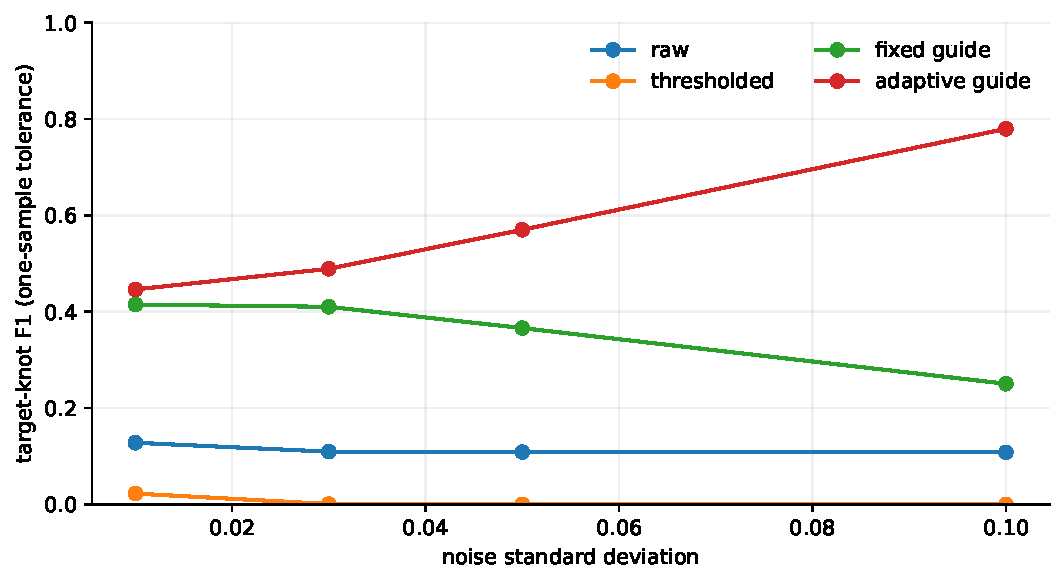
\includegraphics[width=0.92\linewidth]{figures/stability_accuracy.pdf}
\caption{Knot accuracy under repeated Gaussian perturbations.  Stability alone
is insufficient: the thresholded method is stable because it often retains
only endpoints, whereas adaptive guidance retains a compact set of meaningful
knots.}
\label{fig:stability}
\end{figure}

Theorem~\ref{M-thm:persistence} was audited on 1000 seeded perturbations, split
equally between uniform and irregular grids.  No numerical violation occurred;
the maximum observed ratio
$d_{\rm SC}/(C_x\|e\|_\infty)$ was 0.9899.  On the four-sample discontinuity
sequence, hard-baseline amplification grew from 20.5 to approximately
$2\times10^8$ as the curvature scale decreased from $10^{-1}$ to $10^{-8}$,
while the persistence distance remained exactly one half of its theorem bound
up to floating-point error (Figure~\ref{fig:persistence}).

\begin{figure}[H]
\centering
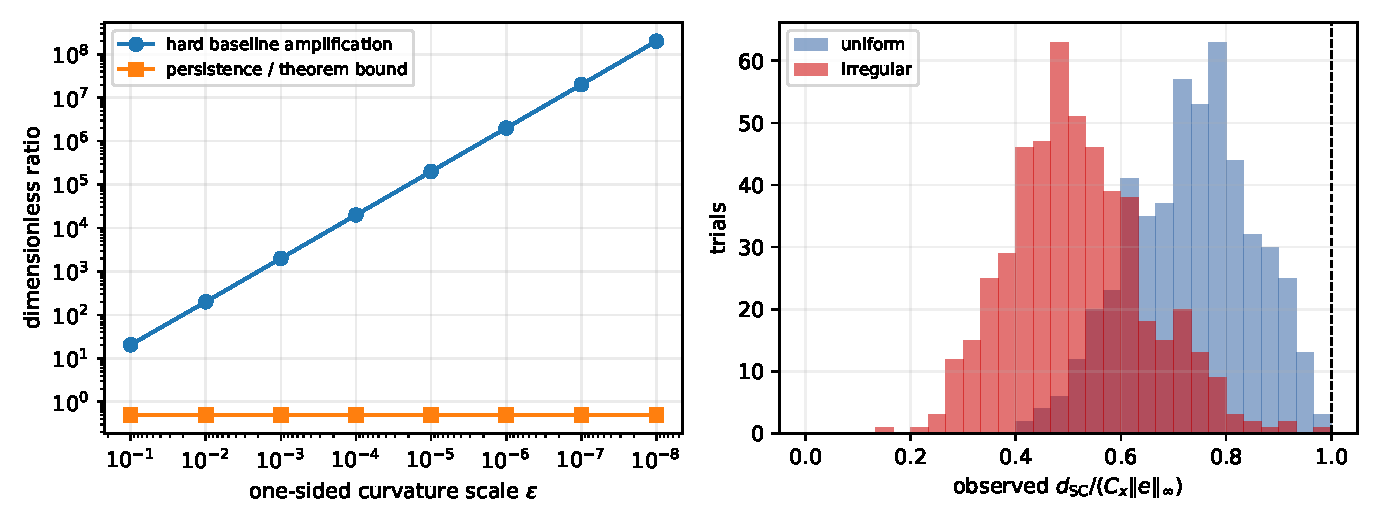
\includegraphics[width=0.96\linewidth]{figures/persistence_stability.pdf}
\caption{Hard-decision discontinuity versus signed-curvature persistence.
Left: the hard baseline has unbounded amplification while the persistence
distance remains within its global bound.  Right: all 1000 uniform/irregular-grid
checks remain below the theorem limit (dashed line).}
\label{fig:persistence}
\end{figure}


\appendix
\section{Boundary cases and detailed proof edges}
\label{app:proofs}

This appendix expands the combinatorial and stability edges most vulnerable to
off-by-one or hidden-decision assumptions.  All indices below are local indices
in the current eligible knot list; mapping them back to original sample indices
preserves order and nesting.

\begin{lemma}[Progress of a nonterminal centred interval]
\label{lem:progress}
Suppose the current interval starts at eligible index $r$ and the centred walk
closes it at $t$ before the terminal endpoint.  Then $t-r\ge2$.
\end{lemma}
\begin{proof}
Let $p\ge r+1$ be the first active curvature after any insignificant entries.
A nonterminal closure requires a later active curvature $q>p$ of the opposite
sign.  There are three possible selected locations.  The first opposite point
is $q\ge p+1\ge r+2$.  A single eligible zero between the two signs is selected
at one index after the last active point, again at least $p+1$.  On a longer
zero plateau, the last point on the departing side is eligible only when it is
not the first active point; hence it is at least $p+1$.  Otherwise the arriving
side is selected.  The implementation's final spacing guard enforces the same
lower bound in degenerate branches.  Thus every nonterminal case has
$t-r\ge2$.
\end{proof}

\begin{lemma}[Halving recurrence]
\label{lem:halving}
If one level starts with $N\ge1$ eligible intervals and produces $N'$ chord
intervals, then $N'\le\lceil N/2\rceil$.
\end{lemma}
\begin{proof}
The produced intervals are consecutive and partition the $N$ old intervals.
By Lemma~\ref{lem:progress}, every produced interval except possibly the last
contains at least two old intervals.  The last contains at least one.  Hence
$N\ge2(N'-1)+1=2N'-1$, so $N'\le(N+1)/2$ and integrality gives the claim.  If
the last interval also contains at least two, the stronger
$N'\le\lfloor N/2\rfloor$ holds.
\end{proof}

\begin{proof}[Detailed completion of Theorem~\ref{thm:finite} and Corollary~\ref{cor:sparse}]
Every new knot is selected from the current eligible list, so the mapped knot
sets are nested.  Let $N_0=n-1$ and let $N_j$ be the number of intervals after
level $j$.  Lemma~\ref{lem:halving} and the identity
$\lceil\lceil a/2\rceil/2\rceil=\lceil a/4\rceil$ give inductively
$N_j\le\lceil N_0/2^j\rceil$.  For $n\ge3$, choosing
$j=\lceil\log_2(n-1)\rceil$ makes $N_j=1$, so the endpoint chord has been
recorded and the implementation stops.  For $n=2$, it records that chord in
one level.  This proves the stated
$\max\{1,\lceil\log_2(n-1)\rceil\}$ bound.  If a sparse implementation spends
$O(N_j)$ work at level $j$, the geometric recurrence gives $O(n)$ total work.
More explicitly, for integer $N_0\ge1$,
$\lceil N_0/2^j\rceil\le(N_0-1)/2^j+1$, so
$\sum_{j=1}^J N_j<N_0-1+J\le2N_0$.  Adding one endpoint per stored knot set
gives $\sum_{j=1}^J|K_j|<2N_0+J$, the stated storage bound.  This is the
complexity of the implemented knot-only representation; materializing every
length-$n$ level remains $O(n\log n)$ in the worst case.
\end{proof}

\begin{lemma}[Centred decision margin]
\label{lem:decision}
On a uniform grid of spacing $h$, define $\gamma$ and $\eta$ as in
Theorem~\ref{thm:local-stability}.
If
$\|e\|_\infty<\min\{\gamma h/4,\eta h/8\}$, every curvature sign and every
adjacent opposite-sign magnitude comparison made by the centred walk is
unchanged.
\end{lemma}
\begin{proof}
The divided-curvature perturbation stencil is
$(1,-2,1)/h$, so every coordinate changes by at most
$4\|e\|_\infty/h$.  The first strict inequality prevents zero crossing.  For
two curvature coordinates $a,b$, the reverse triangle inequality gives
\[
\left|(|a+\delta a|-|b+\delta b|)-(|a|-|b|)\right|
\le |\delta a|+|\delta b|
\le8\|e\|_\infty/h.
\]
The second strict inequality therefore preserves every comparison outcome.
Once signs are fixed there are no zero-curvature branches, and the potential
comparison pairs are the adjacent entries across sign-run boundaries.  These
data determine the same knot walk.
\end{proof}

\begin{proof}[Detailed completion of Theorem~\ref{thm:local-stability}]
Lemma~\ref{lem:decision} fixes the knot set.  At any sample between two fixed
knots, the interpolation error is a convex combination of the two endpoint
errors and is therefore at most $\|e\|_\infty$.  This proves the baseline
bound.  The detail perturbation is $e-[T(y+e)-Ty]$, so the triangle inequality
gives the factor two.  If $\eta=0$, no positive centred-rule radius follows:
the explicit $(1,1,-1)$ counterexample in the main text changes the selected
side while preserving every sign.
\end{proof}

\begin{lemma}[Essential class in the signed persistence metric]
\label{lem:essential}
For a nonempty connected finite path, the ordinary zero-dimensional superlevel
diagram has exactly one essential class.  Under a finite-cost bottleneck
matching between two functions on that path, the essential classes match each
other; the remaining matching restricts to their finite diagrams.
\end{lemma}
\begin{proof}
At the bottom of the filtration the entire path is present and connected, so
exactly one component survives indefinitely.  A diagram point with an infinite
death coordinate has infinite distance from the diagonal and from every finite
point.  Therefore any finite-cost matching pairs the two essential points.
Their cost is the absolute difference of their birth heights, which are the
two function maxima.  Removing that pair leaves precisely a matching of the
finite parts.
\end{proof}

\begin{proof}[Detailed completion of Theorem~\ref{thm:persistence}]
The $i$th divided-curvature row is
\[
\left(h_{i-1}^{-1},
 -(h_{i-1}^{-1}+h_i^{-1}),h_i^{-1}\right),
\]
whose absolute row sum is $2(h_{i-1}^{-1}+h_i^{-1})$.  Taking the maximum gives
the exact induced $\ell_\infty$ norm $C_x$.  Coordinatewise positive part is
1-Lipschitz, so both signed vertex functions differ by at most
$C_x\|y-z\|_\infty$.  Their piecewise-linear extensions over a common edge
differ by a convex combination of endpoint differences and obey the same bound.
Apply persistence-diagram stability to their negatives, which converts
superlevel filtrations to sublevel filtrations without changing the sup norm.
Lemma~\ref{lem:essential} identifies the essential and finite costs used in
$d_{\rm SC}$.  Taking the maximum over signs proves the metric bound.  Finally,
a finite bar $(b,d)$ has diagonal cost $(b-d)/2$; if its lifetime is strictly
greater than twice the metric bound, a bottleneck matching attaining that bound
cannot send it to the diagonal.
\end{proof}

\begin{proof}[Domain detail for Theorem~\ref{thm:prox}]
For $n\ge3$, the divided-curvature matrix has rank $n-2$: given any target
curvature vector, choose an initial value and slope and integrate the target
curvatures successively to construct a preimage.  Thus $D$ is surjective.
Since a proper $\phi$ has nonempty domain, $\phi\circ D$ is proper; it is closed
and convex by continuity and linearity of $D$.  Adding
$\|y-z\|_2^2/2$ makes the objective coercive and strongly convex, so its
minimizer exists and is unique.  The standard proximal theorem now applies to
$g=\phi\circ D$.  If $P=\operatorname{prox}_g$ is firmly nonexpansive, then so
is $I-P$: writing $d=y-z$ and $p=Py-Pz$, firm nonexpansiveness gives
$\|p\|^2\le\langle p,d\rangle$, which directly implies
\[
\|(I-P)y-(I-P)z\|^2\le
\langle (I-P)y-(I-P)z,y-z\rangle.
\]
Finally, $D\ell=0$ gives
$g(w+\ell)=g(w)$; translating the optimization variable establishes affine
equivariance.  The $n=2$ case has the zero curvature map and is immediate.
\end{proof}


\footnotesize
\setlength{\bibsep}{1pt}
\bibliographystyle{plainnat}
\bibliography{references}
\end{document}
